

%-------------------------------------------------------------------------------
% Dokumenten Klasse
\documentclass[
	final,
	a4paper,
	oneside,
	parskip=full,
	headings=standardclasses,
	headings=big,
	pointednumbers
]{scrartcl}

%-------------------------------------------------------------------------------
% Packete nutzen
\usepackage{ngerman,palatino,setspace}
\usepackage[T1]{fontenc}
\usepackage[utf8]{inputenc}
\usepackage[left=20mm,right=20mm,top=25mm,bottom=25mm]{geometry}
\usepackage{amsmath}
\usepackage{mathtools}
\usepackage{tikz}

\usetikzlibrary{automata, positioning, arrows, shapes}

%{
%\tikzset{
%    ->, % makes the edges directed
%    >=stealth, % makes the arrow heads bold
%    node distance=2cm, % specifies the minimum distance between two nodes. Change if necessary.
%    every state/.style={thick, fill=gray!10}, % sets the properties for each ’state’ node
%    every edge/.append style={line width=0.25mm}, % sets the properties for each ’state’ node
%    initial text=$ $, % sets the text that appears on the start arrow
%}
%}

\tikzset{
    node distance=2cm, % Minimum distance between two nodes. Change if necessary.
    every state/.style={ % Sets the properties for each state
        semithick,
        fill=gray!10
    },
    initial text={}, % No label on start arrow
    double distance=2pt, % Adjust appearance of accept states
    every edge/.style={ % Sets the properties for each transition
        draw,
        ->,>=stealth, % Makes edges directed with bold arrowheads
        auto,
        semithick
    }
}

%-------------------------------------------------------------------------------
\usepackage{multirow}

%-------------------------------------------------------------------------------
% uline
\usepackage{ulem}

%-------------------------------------------------------------------------------
% Anderer Font
\usepackage{mathrsfs}
\usepackage[mathcal]{euscript}

%-------------------------------------------------------------------------------
% Square brackets
\usepackage{stmaryrd}


\newcommand{\newState}[4]{\node[state,#3](#1)[#4]{#2};}
\newcommand{\newTransition}[4]{\path[->] (#1) edge [#4] node {#3} (#2);} 

%-------------------------------------------------------------------------------
% Dokument
\begin{document}
    
    
    %--- Page 1 --------------------------------------------------------------------
    
   	
    \begin{minipage}{0.2\textwidth}
       ab:
   	\end{minipage}
   	\begin{minipage}{0.8\textwidth}
       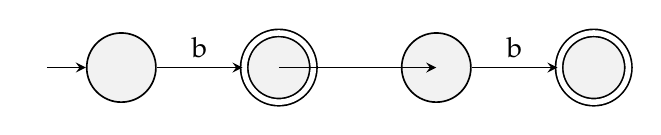
\begin{tikzpicture}
           \node[state, initial left]                  (aq1)    {};
           \node[state, accepting, right of=aq1]       (aq2)    {};
           \node[state, right of=aq2]                  (bq1)    {};
           \node[state, accepting, right of=bq1]       (bq2)    {};
           \coordinate (x) at (aq2);
           \coordinate (y) at (bq1);
           \draw   (aq1) edge[]        node{b} (aq2)
                   (bq1) edge[]        node{b} (bq2)
                   (x) edge (y)
           ;
       \end{tikzpicture}
   	\end{minipage}
       
   	\begin{minipage}{0.2\textwidth}
        ab:
   	\end{minipage}
   	\begin{minipage}{0.8\textwidth}
        \begin{tikzpicture}
            \node[state, initial left]                  (aq1)    {};
            \node[state, accepting, right of=aq1]       (aq2)    {
            \begin{tikzpicture}
                \draw (0,0) -- (0,1);
            \end{tikzpicture}};
            \node[state, right of=aq2]                  (bq1)    {};
            \node[state, accepting, right of=bq1]       (bq2)    {};
            \draw   (aq1) edge[]        node{b} (aq2)
                    (bq1) edge[]        node{b} (bq2)
            ;
        \end{tikzpicture}
   	\end{minipage}


   	\begin{minipage}{0.2\textwidth}
        ab:
   	\end{minipage}
   	\begin{minipage}{0.8\textwidth}
        \def\dx{1cm} 
        \def\dy{1.5cm}
        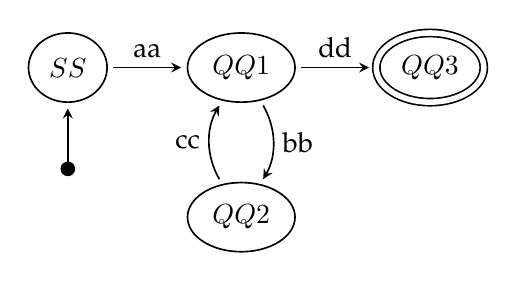
\begin{tikzpicture}[
                every state/.style={draw,ellipse},
                node distance=\dy and \dx,
                >=latex,shorten >=2pt,shorten <=2pt,auto,
                semithick,  %semithick, thick, thin semithick
                initial distance=1cm,
                every initial by arrow/.style={*->}
            ]
            \newState{S}{$SS$}{initial below}{}
            \newState{q1}{$QQ1$}{right=of S}{}
            \newState{q2}{$QQ2$}{below=of q1}{}
            \newState{q3}{$QQ3$}{right=of q1}{accepting} 
            
            \newTransition{S}{q1}{aa}{}
            \newTransition{q1}{q2}{bb}{bend left}
            \newTransition{q2}{q1}{cc}{bend left}
            \newTransition{q1}{q3}{dd}{}
        \end{tikzpicture}
   	\end{minipage}

    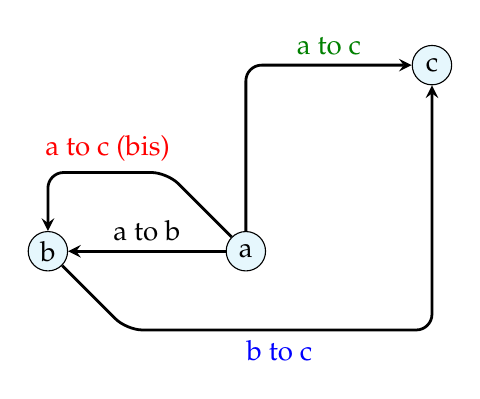
\begin{tikzpicture}[node distance=2cm and 2cm]
        \tikzset{
            sh2n/.style={shift={(0,1)}},
            sh2s/.style={shift={(0,-1)}},
            sh2e/.style={shift={(1,0)}},
            sh2w/.style={shift={(-1,0)}},
            %
            sh2nw/.style={shift={(-1,1)}},
            sh2ne/.style={shift={(1,1)}},
            sh2sw/.style={shift={(-1,-1)}},
            sh2se/.style={shift={(1,-1)}},
            %
            rc/.style={rounded corners=2mm,line width=1pt},
            %
            place/.style={draw,circle,fill=cyan!10,inner sep=.5mm,minimum size=5mm},
        }
        \node[place] (a) {a};
        \node[place,left=of a] (b) {b};
        \node[place,above right=of a] (c) {c};
        
        \draw[-stealth,rc] (a) -- node[above]{a to b} (b);
        \draw[-stealth,rc] (a) |- node[green!50!black,above,pos=.75]{a to c} (c);
        \draw[-stealth,rc] (a) -- ([sh2nw]a.center) -- node[above,red] {a to c (bis)} ([sh2n]b.center) -- (b);
        \draw[-stealth,rc] (b) -- ([sh2se]b.center) -| node[below,blue,pos=.25] {b to c} (c);
    \end{tikzpicture}

\end{document}
